\graphicspath{ {images/} }

\titledquestion{Position Embeddings Exploration}[6]
\label{sec:pos_enc}

Position embeddings are an important component of the Transformer architecture, allowing the model to differentiate between tokens based on their position in the sequence.
In this question, we'll explore the need for positional embeddings in Transformers and how they can be designed.

Recall that the crucial components of the Transformer architecture are the self-attention layer and the feed-forward neural network layer. 
Given an input tensor $\mathbf{X} \in \mathbb{R}^{T \times d}$, where $T$ is the sequence length and $d$ is the hidden dimension, the self-attention layer computes the following:
\begin{align*}
    \mathbf{Q} &= \mathbf{X}\mathbf{W}_Q, \quad \mathbf{K} = \mathbf{X}\mathbf{W}_K, \quad \mathbf{V} = \mathbf{X}\mathbf{W}_V \\
    \mathbf{H} &= \text{softmax}\left(\frac{\mathbf{Q}\mathbf{K}^{\top}}{\sqrt{d}}\right) \mathbf{V}
\end{align*}
where $\mathbf{W}_Q, \mathbf{W}_K, \mathbf{W}_V \in \mathbb{R}^{d \times d}$ are weight matrices, and $\mathbf{H} \in \mathbb{R}^{T \times d}$ is the output.

Next, the feed-forward layer applies the following transformation:
\begin{align*}
    \mathbf{Z} = \text{ReLU}(\mathbf{H}\mathbf{W}_1 + \mathbf{1}\cdot\mathbf{b}_1)\mathbf{W}_2 + \mathbf{1}\cdot\mathbf{b}_2
\end{align*}
where $\mathbf{W}_1, \mathbf{W}_2 \in \mathbb{R}^{d \times d}$ and $\mathbf{b}_1, \mathbf{b}_2 \in \mathbb{R}^{1\times d}$ are weights and biases; $\mathbf{1} \in \mathbb{R}^{T\times 1}$ is a vector of ones\footnote{Outer product with $\mathbf{1}$ represents broadcasting operation and makes feed forward network notations mathematically sound.}; and $\mathbf{Z} \in \mathbb{R}^{T \times d}$ is the final output.

(Note that we have omitted some details of the Transformer architecture for simplicity.)

\begin{parts}
    \part[4] \textbf{Permuting the input.}
    
    \begin{subparts}
        \subpart[3]
        Suppose we permute the input sequence $\mathbf{X}$ such that the tokens are shuffled randomly. This can be represented as multiplication by a permutation matrix $\mathbf{P} \in \mathbb{R}^{T \times T}$, i.e. $\mathbf{X}_{\text{perm}} = \mathbf{P}\mathbf{X}$. (See \href{https://en.wikipedia.org/wiki/Permutation_matrix}{Wikipedia} for a recap on permutation matrices.)

        \textbf{Show} that the output $\mathbf{Z}_{\text{perm}}$ for the permuted input $\mathbf{X}_{\text{perm}}$ will be $\mathbf{Z}_{\text{perm}} = \mathbf{P}\mathbf{Z}$.

        You are given that for any permutation matrix $\mathbf{P}$ and any matrix $\mathbf{A}$, the following hold:
        $\text{softmax}(\mathbf{P}\mathbf{A}\mathbf{P}^{\top}) = \mathbf{P}\ \text{softmax}(\mathbf{A})\ \mathbf{P}^{\top} \quad \text{and}\quad \text{ReLU}(\mathbf{P}\mathbf{A}) = \mathbf{P}\ \text{ReLU}(\mathbf{A})$.

        \ifans{
            \newline
            Given an input tensor $\mathbf{X} \in \mathbb{R}^{T \times d}$, a permutation matrix $\mathbf{P} \in \mathbb{R}^{T \times T}$ is applied to shuffle the rows of $\mathbf{X}$ along the time axis (i.e., the sequence dimension). First, we linearly project the permuted input matrix $\mathbf{X}_{\text{perm}}$ to $\mathbf{Q}_{\text{perm}}$, $\mathbf{K}_{\text{perm}}$, and $\mathbf{V}_{\text{perm}}$ as follows:
            $$
                \mathbf{Q}_{\text{perm}} = \mathbf{PX}\mathbf{W}_Q, 
                \quad \mathbf{K}_{\text{perm}} = \mathbf{PX}\mathbf{W}_K, 
                \quad \mathbf{V}_{\text{perm}} = \mathbf{PX}\mathbf{W}_V \\
            $$

            Then, the output of the self-attention layer is defined as:
            \begin{align*}
                \mathbf{H}_{\text{perm}}
                &= \text{softmax}(\frac{\mathbf{Q}_{\text{perm}}\mathbf{K}_{\text{perm}}^\top}{\sqrt{d}}) \mathbf{V}_{\text{perm}} \\
                &= \text{softmax}(\frac{\mathbf{PX}\mathbf{W}_Q \mathbf{W}_K^\top \textbf{X}^\top \textbf{P}^\top}{\sqrt{d}}) \mathbf{V}_{\text{perm}} \\
                &= \text{softmax}(\mathbf{P}\frac{\mathbf{X}\mathbf{W}_Q \mathbf{W}_K^\top \mathbf{X}^\top}{\sqrt{d}} \mathbf{P}^\top) \mathbf{V}_{\text{perm}} \\
                &= \text{softmax}(\mathbf{P}\frac{\mathbf{X}\mathbf{W}_Q (\mathbf{X}\mathbf{W}_K)^\top}{\sqrt{d}} \mathbf{P}^\top) \mathbf{V}_{\text{perm}} \\
                &= \text{softmax}(\mathbf{P}\frac{\mathbf{X}\mathbf{W}_Q (\mathbf{X}\mathbf{W}_K)^\top}{\sqrt{d}} \mathbf{P}^\top) \mathbf{V}_{\text{perm}} \\
                &= \mathbf{P} \text{softmax}\left(\frac{\mathbf{Q}\mathbf{K}^{\top}}{\sqrt{d}}\right) \mathbf{P}^\top \mathbf{PX}\mathbf{W}_V \\
                &= \mathbf{P} \text{softmax}\left(\frac{\mathbf{Q}\mathbf{K}^{\top}}{\sqrt{d}}\right) \mathbf{IX}\mathbf{W}_V \quad\quad \because \mathbf{P}^\top = \mathbf{P}^{-1} \\
                &= \mathbf{P} \text{softmax}\left(\frac{\mathbf{Q}\mathbf{K}^{\top}}{\sqrt{d}}\right) \mathbf{IV} \\
                &= \mathbf{PH}
            \end{align*}

            After the self-attention layer, we feed $\mathbf{H}_{\text{perm}}$ into the position-wise feed-forward network as follows:
            \begin{align*}
                \mathbf{Z}_{\text{perm}}
                &= \text{ReLU}(\mathbf{PH}\mathbf{W}_1 + \mathbf{1}\cdot\mathbf{b}_1)\mathbf{W}_2 + \mathbf{1}\cdot\mathbf{b}_2 \\
                &= \text{ReLU}(\mathbf{PH}\mathbf{W}_1 + \mathbf{P}(\mathbf{1}\cdot\mathbf{b}_1))\mathbf{W}_2 + \mathbf{1}\cdot\mathbf{b}_2 \quad\quad \because \mathbf{b}_1 \text{ is broadcast to all time steps.} \\
                &= \text{ReLU}(\mathbf{P}(\mathbf{H}\mathbf{W}_1 + \mathbf{1}\cdot\mathbf{b}_1))\mathbf{W}_2 + \mathbf{1}\cdot\mathbf{b}_2 \\
                &= \mathbf{P} \text{ReLU}(\mathbf{H}\mathbf{W}_1 + \mathbf{1}\cdot\mathbf{b}_1)\mathbf{W}_2 + \mathbf{1}\cdot\mathbf{b}_2 \\
                &= \mathbf{P} \text{ReLU}(\mathbf{H}\mathbf{W}_1 + \mathbf{1}\cdot\mathbf{b}_1)\mathbf{W}_2 + \mathbf{1}\cdot\mathbf{b}_2 \\
                &= \mathbf{P} \text{ReLU}(\mathbf{H}\mathbf{W}_1 + \mathbf{1}\cdot\mathbf{b}_1)\mathbf{W}_2 + \mathbf{P}(\mathbf{1}\cdot\mathbf{b}_2) \quad\quad \because \mathbf{b}_2 \text{ is broadcast to all time steps.} \\
                &= \mathbf{P}[\text{ReLU}(\mathbf{H}\mathbf{W}_1 + \mathbf{1}\cdot\mathbf{b}_1)\mathbf{W}_2 + \mathbf{1}\cdot\mathbf{b}_2] \\
                &= \mathbf{PZ}
            \end{align*}

            Hence, we get $\mathbf{Z}_{\text{perm}} = \mathbf{PZ}$ for a given $\mathbf{X}_{\text{perm}} = \mathbf{PX}$.
        }
        \subpart[1] Think about the implications of the result you derived in part i. \textbf{Explain} why this property of the Transformer model could be problematic when processing text.

        \ifans{
            \newline
            The most notable property of a transformer block (which consists of a self-attention layer followed by a position-wise feed-forward layer) is that it can only approximate \textbf{permutation equivariant} functions. In simpler terms, the output of the transformer block changes correspondingly just as how the input sequence is rearranged (i.e., permuted). However, this poses a challenge: it disregards the order of the sequence, which hinders the model from capturing the inherent sequential structure of the text.
        }
    \end{subparts}

    \part[2] \textbf{Position embeddings} are vectors that encode the position of each token in the sequence. They are added to the input word embeddings before feeding them into the Transformer.

    One approach is to generate position embedding using a fixed function of the position and the dimension of the embedding. If the input word embeddings are $\mathbf{X} \in \mathbb{R}^{T \times d}$, the position embeddings $\Phi \in \mathbb{R}^{T \times d}$ are generated as follows:
    \begin{align*}
        \Phi_{(t, 2i)} &= \sin\left({t}/{10000^{2i/d}}\right) \\
        \Phi_{(t, 2i+1)} &= \cos\left({t}/{10000^{2i/d}}\right)
    \end{align*}
    where $t \in \{0, 1, \ldots T-1\}$ and $i \in \{0, 1, \ldots d/2-1\}$\footnote{Here $d$ is assumed even which is typically the case for most models.}.

    Specifically, the position embeddings are added to the input word embeddings:
    \begin{align*}
        \mathbf{X}_{\text{pos}} = \mathbf{X} + \Phi
    \end{align*}

    \begin{subparts}
        \subpart[1] Do you think the position embeddings will help the issue you identified in part (a)? If yes, explain how and if not, explain why not.

        \ifans{
            \newline
            By adding the absolute position embeddings to the input token embeddings, each position is marked with an unique position identifier. The injected position information enables the model to infer the relative distances among different tokens. Also, it lets the model treat the sequence as an ordered structure, rather than an unordered set of tokens.
        }
        \subpart[1] Can the position embeddings for two different tokens in the input sequence be the same? If yes, provide an example. If not, explain why not.

        \ifans{
            \newline
            Figure \ref{fig2} illustrates positional encodings with different bases. Collisions occur more frequently with smaller bases, while larger bases yield more unique encodings for different positions. However, collisions can still arise with a small embedding dimension $d$, as \textbf{higher angular frequencies} dominate the early dimensions.
            
            \begin{figure}[H]
            \centering
            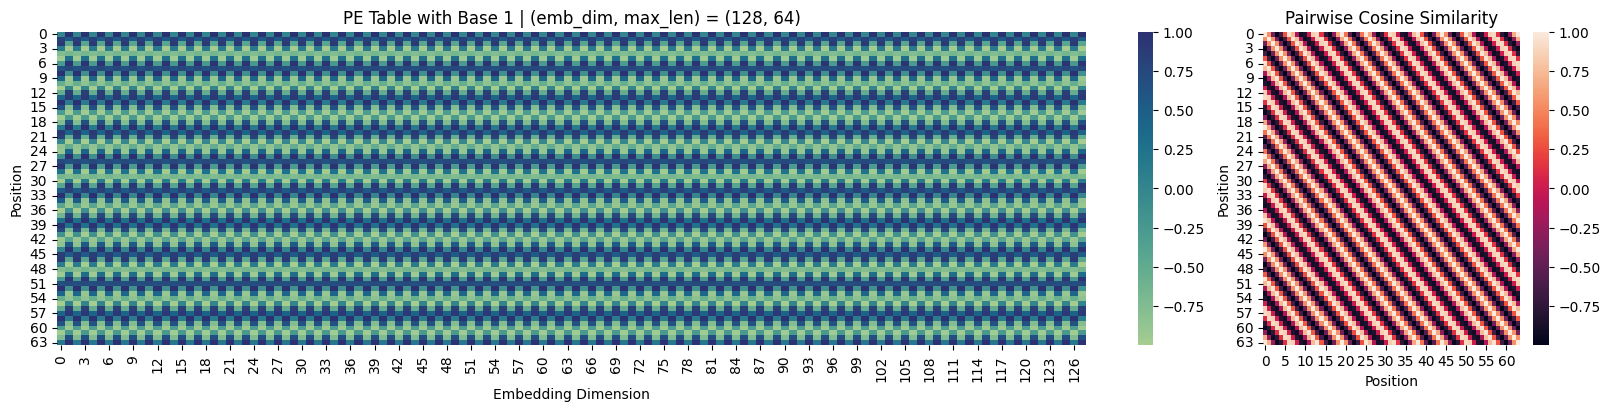
\includegraphics[width=\textwidth]{assets/pe_1.png}
            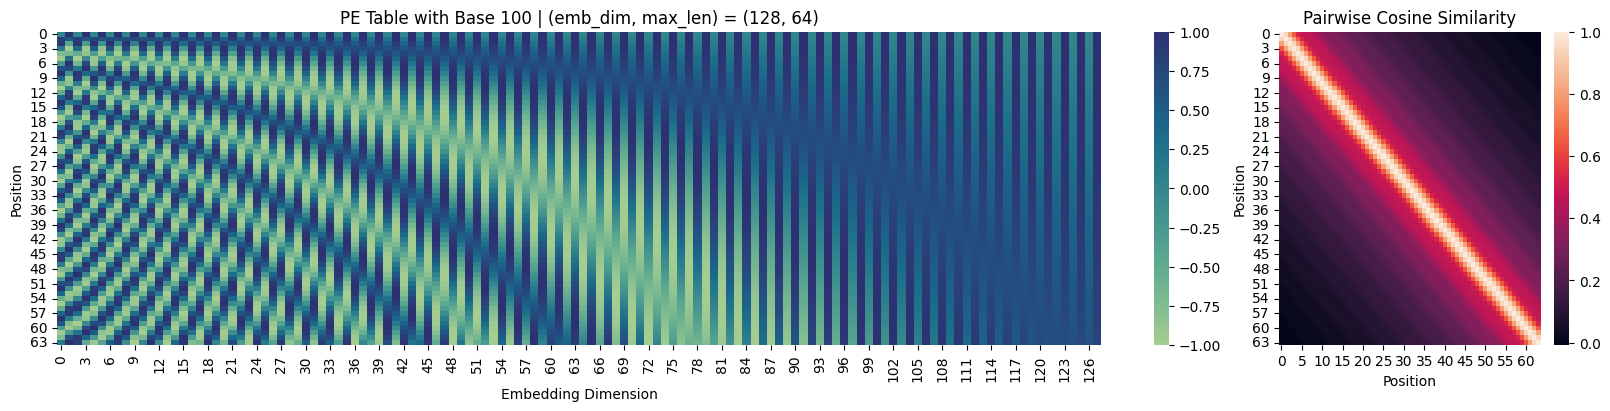
\includegraphics[width=\textwidth]{assets/pe_100.png}
            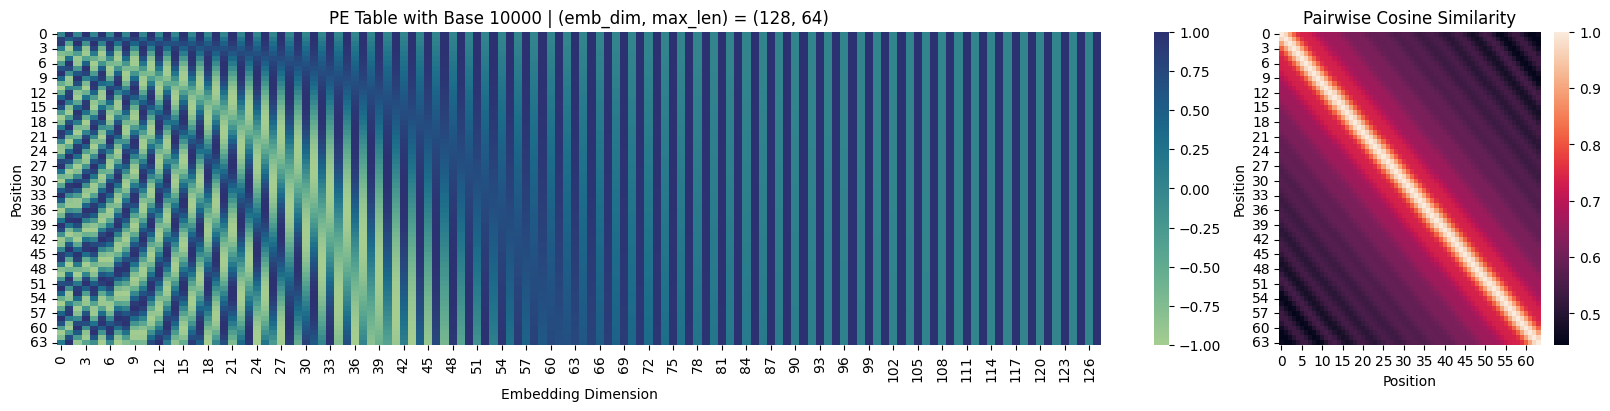
\includegraphics[width=\textwidth]{assets/pe_10000.png}
            \caption{Positional encodings with different bases.}
            \label{fig2}
            \end{figure}
            
        }
    \end{subparts}
\end{parts}








































































































































